\chapter{Results}\label{chapter_results}

This Chapter is concerned with the presentation of the results obtained from a practical
application of the algorithms implemented in
Chapter~\ref{chapter_implementation} on various image sequences. 
The image sequences are mainly taken from the Visual Object Tracking 2017
Challenge (VOT2017)~\cite{VOT2017}. The famous Hamburg taxi
sequence~\cite{Hamburg} is also used as an
initial experiment for the template matching trackers.

The analysis of the algorithms is both quantitative and qualitative as defined
in Section~\ref{methodology_testing}. The
quantitative analysis is based on the tracker performance per the defined centroid
``tracker error'' metric. The qualitative analysis is based on both the metric
and experts of bounding boxes, it aims to provide an insight into the results
based on the data informed by an understanding of the various algorithm
implementations. 

This Chapter also presents the results of the overall integrated MT System, and
gauges it's performance by relating it back to the system
s user requirements stated in Section~\ref{introduction_user_requirements}.


\section{Template Matching Tracker}
This Section presents a qualitative and quantitative (where applicable) analysis
of the performance of the simple and
adaptive template tracker variants (STT and ATT respectively) that were proposed
in Section~\ref{theoretical_framework_tm}. 

Both trackers were applied to the Hamburg taxi sequence  as an initial
test of their applicability to the motion tracking problem.
The template trackers below were run for a threshold $\tau=0.8$.

\subsection{Simple template matching tracker}\label{results_simple_template_matching}
In Figure~\ref{fig:simple_template_tracking} the initial user selected template used for matching is the shown by the rectangular region around the car
in the first frame. The images shown correspond to almost equally spaced
samples of the 40 frame taxi sequence.

It can be seen that the STT manages to track the car
up until $\mathbf{F}_{6}$ in the Figure, corresponding to $\mathbf{f}_{12}$ in
the sequence, beyond which the rotation of the car drives the sum of square
differences similarity measure between the initial template chosen in
$\mathbf{f}_0$ and the region of interest in $\mathbf{f}_{12}$ below the
threshold.

It is important to highlight that, while lowering the detection threshold allows
the tracker to follow the car for a larger amount of frames, this is not a
solution to the problem as the tracker becomes more susceptible to noise, and is
certainly not a good model for robustness across different sequences.

An idea to get around the changing template, is the implementation of an
adaptive template matching algorithm, in which we update the model we are
looking for each $\mathbf{f}_k$.



\begin{figure}    
    \makebox[\linewidth][c]{
    \begin{tabular}{cccc}
        \subfloat{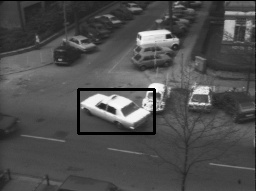
\includegraphics[width = 1.5in]{figures/results/simple_template_tracker/taxi_sequence/1.jpg}} &
        \subfloat{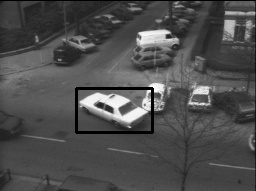
\includegraphics[width = 1.5in]{figures/results/simple_template_tracker/taxi_sequence/2.jpg}} &
        \subfloat{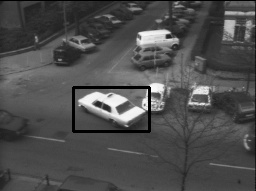
\includegraphics[width = 1.5in]{figures/results/simple_template_tracker/taxi_sequence/3.jpg}} &
        \subfloat{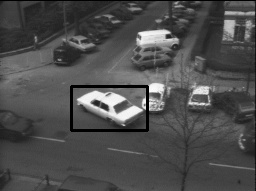
\includegraphics[width = 1.5in]{figures/results/simple_template_tracker/taxi_sequence/4.jpg}} \\

        \subfloat{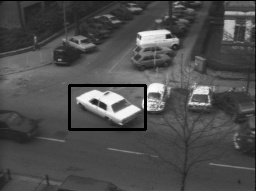
\includegraphics[width = 1.5in]{figures/results/simple_template_tracker/taxi_sequence/5.jpg}} &
        \subfloat{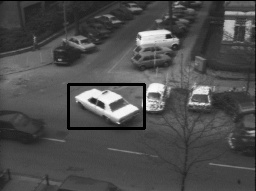
\includegraphics[width = 1.5in]{figures/results/simple_template_tracker/taxi_sequence/6.jpg}} &
        \subfloat{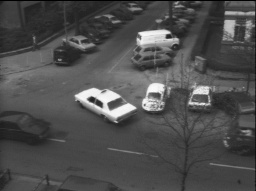
\includegraphics[width = 1.5in]{figures/results/simple_template_tracker/taxi_sequence/7.jpg}} &
        \subfloat{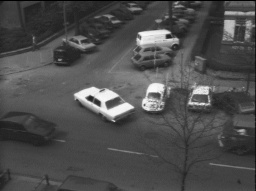
\includegraphics[width = 1.5in]{figures/results/simple_template_tracker/taxi_sequence/8.jpg}} \\
       
        \subfloat{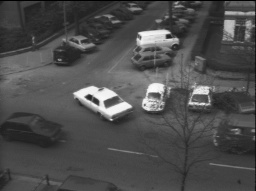
\includegraphics[width = 1.5in]{figures/results/simple_template_tracker/taxi_sequence/9.jpg}} &
        \subfloat{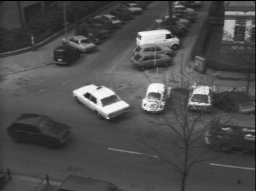
\includegraphics[width = 1.5in]{figures/results/simple_template_tracker/taxi_sequence/10.jpg}} &
        \subfloat{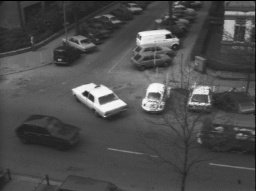
\includegraphics[width = 1.5in]{figures/results/simple_template_tracker/taxi_sequence/11.jpg}} &
        \subfloat{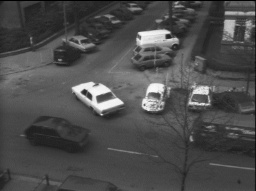
\includegraphics[width = 1.5in]{figures/results/simple_template_tracker/taxi_sequence/12.jpg}} \\
       
        \subfloat{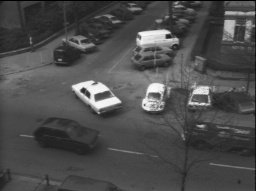
\includegraphics[width = 1.5in]{figures/results/simple_template_tracker/taxi_sequence/13.jpg}} &
        \subfloat{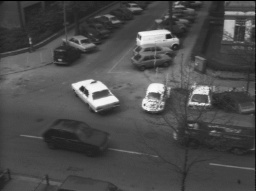
\includegraphics[width = 1.5in]{figures/results/simple_template_tracker/taxi_sequence/14.jpg}} &
        \subfloat{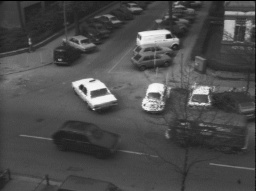
\includegraphics[width = 1.5in]{figures/results/simple_template_tracker/taxi_sequence/15.jpg}} &
        \subfloat{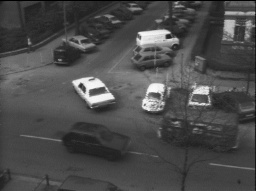
\includegraphics[width = 1.5in]{figures/results/simple_template_tracker/taxi_sequence/16.jpg}} \\   

        \end{tabular}}
    \caption{Simple template tracker applied to Hamburg taxi sequence\label{fig:simple_template_tracking}}
\end{figure}

\subsection{Adaptive template matching tracker}\label{results_adaptive_template_matching}
As described in Section~\ref{theoretical_framework_tm}, the assumption
that an object maintains the same appearance is only valid for an interval of
$K$ frames. Beyond this interval, the template from $\mathbf{f}_{k}$ is sufficiently different
from the object to be matched in $\mathbf{f}_{k+K}$ such that the similarity
measure falls below $\tau$. For the experiments a threshold of $\tau=0.8$ was used.

The idea behind the ATT is that we update the template which we are trying to
match before the we traverse more than
$K$ frames.

\subsubsection{Hamburg taxi sequence}
The sequence in Figure~\ref{fig:adaptive_template_tracking} is generated by
updating the template every frame, the located object in frame,
$\mathbf{f}_{k-1}$. becomes the template for $\mathbf{f}_k$.

From Figure~\ref{fig:adaptive_template_tracking} it shows that the ATT manages
to locate the car within a bounding box in each frame of the sequence. It should
however be noted that there is a noticeable ``drift'' in
the localisation. 
This is due to the fact that the algorithm has no way of controlling the amount of
background noise that is allowed into the template.

\begin{figure}     
    \makebox[\linewidth][c]{
    \begin{tabular}{cccc}
        \subfloat{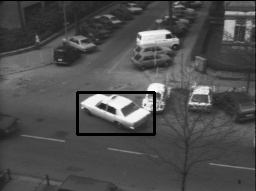
\includegraphics[width = 1.5in]{figures/results/adaptive_template_tracker/taxi_sequence/1.jpg}} &
        \subfloat{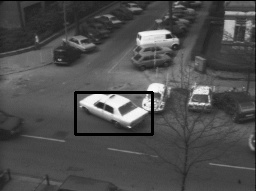
\includegraphics[width = 1.5in]{figures/results/adaptive_template_tracker/taxi_sequence/2.jpg}} &
        \subfloat{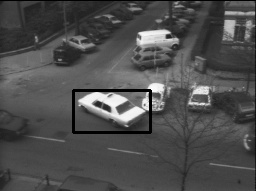
\includegraphics[width = 1.5in]{figures/results/adaptive_template_tracker/taxi_sequence/3.jpg}} &
        \subfloat{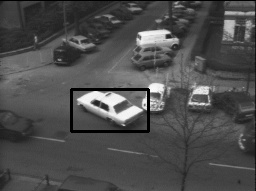
\includegraphics[width = 1.5in]{figures/results/adaptive_template_tracker/taxi_sequence/4.jpg}} \\

        \subfloat{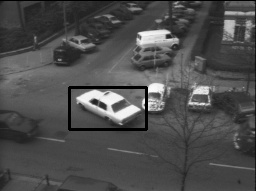
\includegraphics[width = 1.5in]{figures/results/adaptive_template_tracker/taxi_sequence/5.jpg}} &
        \subfloat{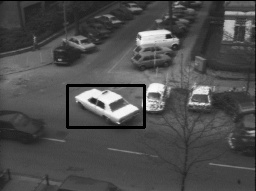
\includegraphics[width = 1.5in]{figures/results/adaptive_template_tracker/taxi_sequence/6.jpg}} &
        \subfloat{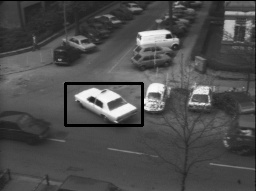
\includegraphics[width = 1.5in]{figures/results/adaptive_template_tracker/taxi_sequence/7.jpg}} &
        \subfloat{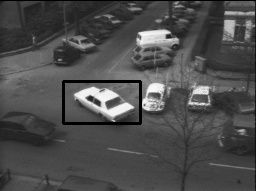
\includegraphics[width = 1.5in]{figures/results/adaptive_template_tracker/taxi_sequence/8.jpg}} \\
       
        \subfloat{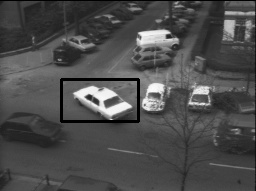
\includegraphics[width = 1.5in]{figures/results/adaptive_template_tracker/taxi_sequence/9.jpg}} &
        \subfloat{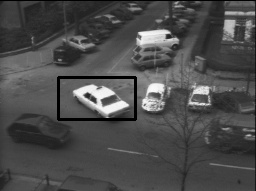
\includegraphics[width = 1.5in]{figures/results/adaptive_template_tracker/taxi_sequence/10.jpg}} &
        \subfloat{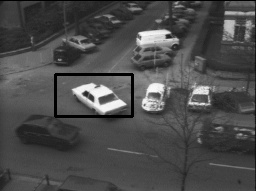
\includegraphics[width = 1.5in]{figures/results/adaptive_template_tracker/taxi_sequence/11.jpg}} &
        \subfloat{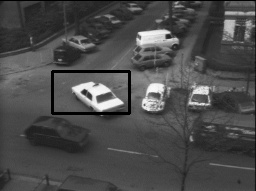
\includegraphics[width = 1.5in]{figures/results/adaptive_template_tracker/taxi_sequence/12.jpg}} \\
       
        \subfloat{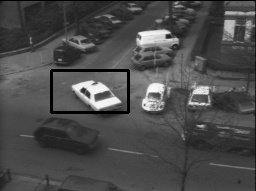
\includegraphics[width = 1.5in]{figures/results/adaptive_template_tracker/taxi_sequence/13.jpg}} &
        \subfloat{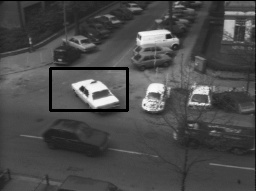
\includegraphics[width = 1.5in]{figures/results/adaptive_template_tracker/taxi_sequence/14.jpg}} &
        \subfloat{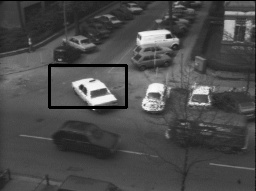
\includegraphics[width = 1.5in]{figures/results/adaptive_template_tracker/taxi_sequence/15.jpg}} &
        \subfloat{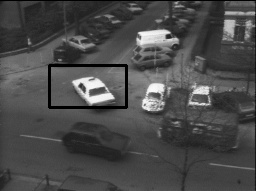
\includegraphics[width = 1.5in]{figures/results/adaptive_template_tracker/taxi_sequence/16.jpg}} \\   

        \end{tabular}}
    \caption{Adaptive template tracker applied to Hamburg taxi sequence\label{fig:adaptive_template_tracking}}
\end{figure}

\subsubsection{Adaptive template tracker vs occlusion}
The graph in Figure~\ref{fig:results/adaptive_template_tracker/metric}, shows the
performance of the MST according to the tracking error metric outlined in
Section~\ref{methodology_testing}. 

Figure~\ref{fig:adaptive_template_occlusion} shows the visual bounding box and
underlying template used for the data in presented in the graph. $\mathbf{F}_{13}$ to
$\mathbf{F}_{16}$ detail the point of failure. As the girl crosses in front of
the man, the adaptive template is updated with information from the man in the
background which as the girl moves away becomes the larger match, thus the
tracker loses the girl. 

\Figure[width=0.8\columnwidth]{Graph of tracker error of ATT (pixels) vs frames in sequence}{results/adaptive_template_tracker/metric}

\begin{figure}     
    \makebox[\linewidth][c]{
    \begin{tabular}{cccc}
        \subfloat{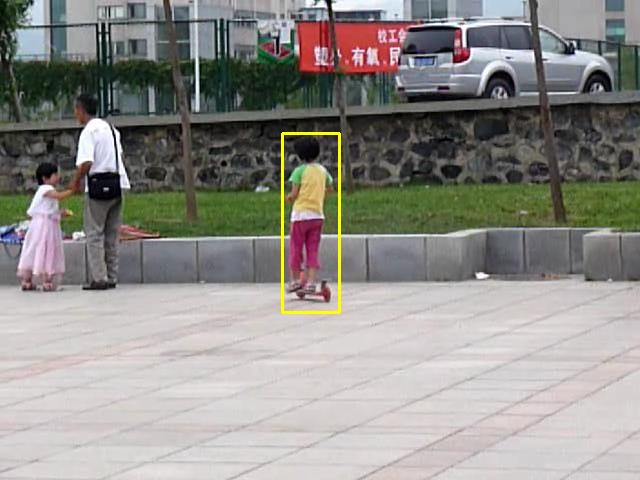
\includegraphics[width = 1.5in]{figures/results/adaptive_template_tracker/girl/2.jpg}} &
        \subfloat{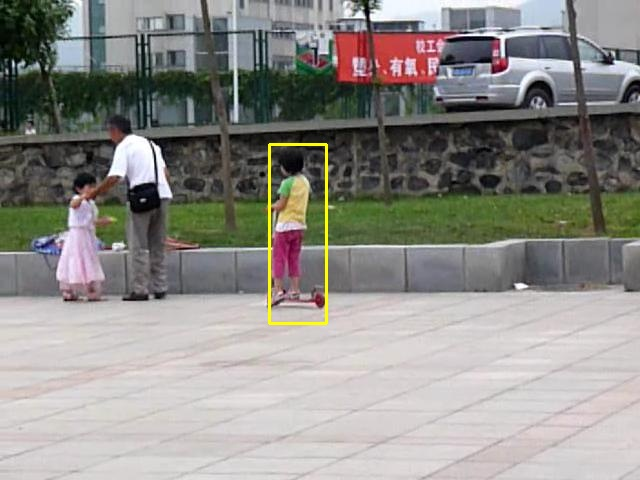
\includegraphics[width = 1.5in]{figures/results/adaptive_template_tracker/girl/3.jpg}} &
        \subfloat{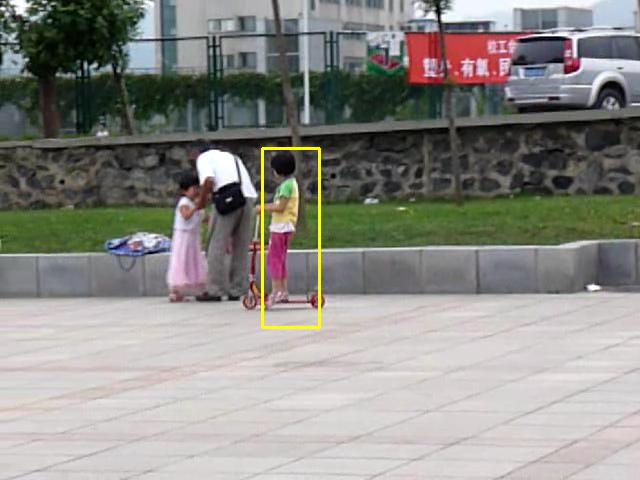
\includegraphics[width = 1.5in]{figures/results/adaptive_template_tracker/girl/4.jpg}} &
        \subfloat{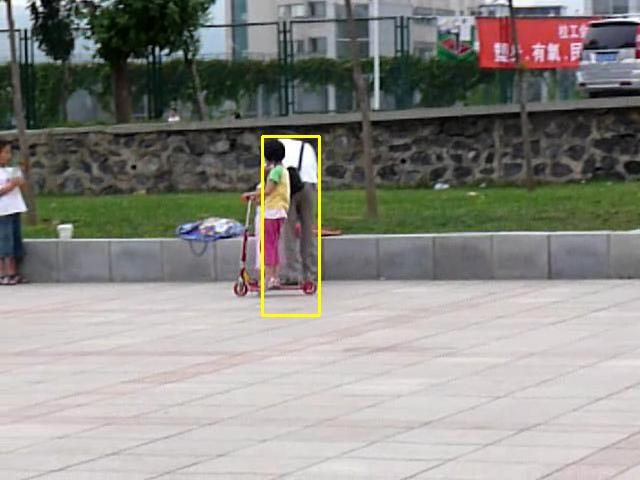
\includegraphics[width = 1.5in]{figures/results/adaptive_template_tracker/girl/5.jpg}} \\

        \subfloat{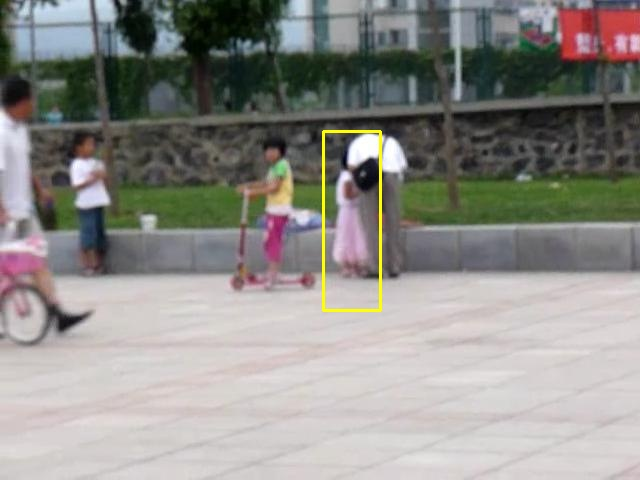
\includegraphics[width = 1.5in]{figures/results/adaptive_template_tracker/girl/6.jpg}} &
        \subfloat{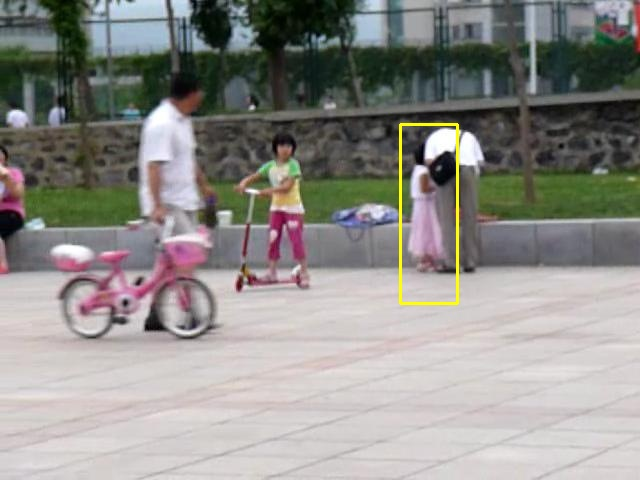
\includegraphics[width = 1.5in]{figures/results/adaptive_template_tracker/girl/7.jpg}} &
        \subfloat{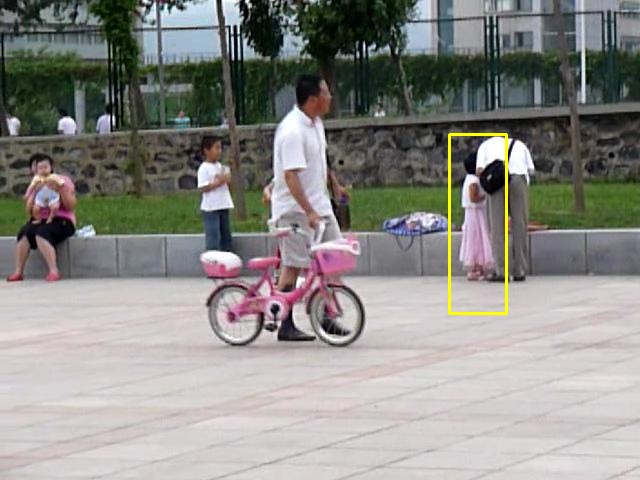
\includegraphics[width = 1.5in]{figures/results/adaptive_template_tracker/girl/8.jpg}} &
        \subfloat{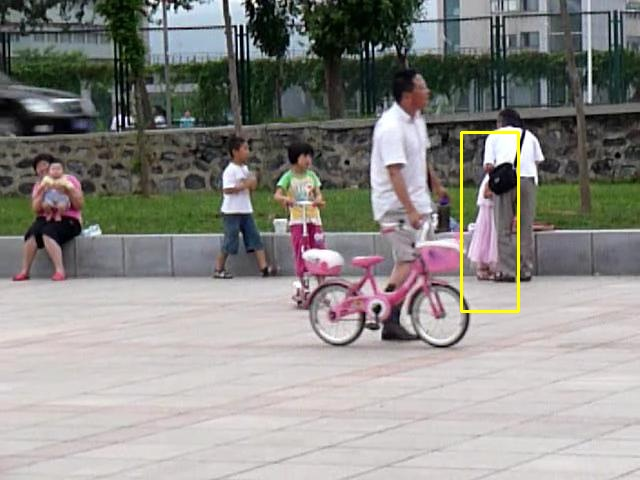
\includegraphics[width = 1.5in]{figures/results/adaptive_template_tracker/girl/9.jpg}} \\
       
        \subfloat{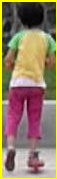
\includegraphics[width = 0.3in]{figures/results/adaptive_template_tracker/girl/10.jpg}} &
        \subfloat{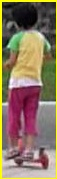
\includegraphics[width = 0.3in]{figures/results/adaptive_template_tracker/girl/11.jpg}} &
        \subfloat{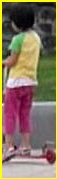
\includegraphics[width = 0.3in]{figures/results/adaptive_template_tracker/girl/12.jpg}} &
        \subfloat{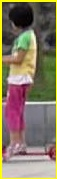
\includegraphics[width = 0.3in]{figures/results/adaptive_template_tracker/girl/13.jpg}} \\
       
        \subfloat{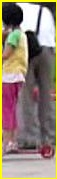
\includegraphics[width = 0.3in]{figures/results/adaptive_template_tracker/girl/14.jpg}} &
        \subfloat{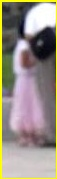
\includegraphics[width = 0.3in]{figures/results/adaptive_template_tracker/girl/15.jpg}} &
        \subfloat{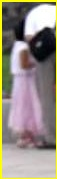
\includegraphics[width = 0.3in]{figures/results/adaptive_template_tracker/girl/16.jpg}} &
        \subfloat{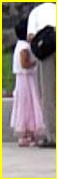
\includegraphics[width = 0.3in]{figures/results/adaptive_template_tracker/girl/17.jpg}} \\   

        \end{tabular}}
    \caption{Subsequence showing ATT performance when faced with occlusion\label{fig:adaptive_template_occlusion}}
\end{figure}

From the graph in Figure~\ref{fig:adaptive_template_occlusion} we can
quantitative observe tracker drift (as was also the case in the Hamburg taxi
sequence) by the steady growth of the average tracker error between
$\mathbf{f}_0$ and $\mathbf{f}_{40}$ before failing completely.
Before it loses track of the girl, the tracker has an average tracking error of
6 pixels between the tracked center and that of the ground truth values.

Depending on it's similarity threshold $\tau$, the adaptive template tracker
either fails to locate the object in the case of a larger $\tau$ and rapid
occlusion between successive frames, $\mathbf{f}_k$ and $\mathbf{f}_{k+1}$ or
adds the occlusion to the target model in the case of a lower $\tau$, and a
slowly progressing occlusion between $\mathbf{f}_k$ and $\mathbf{f}_{k+1}$, as
is the case in Figure~\ref{fig:adaptive_template_occlusion}, where the frames
and their corresponding target models (updated templates) are shown. 

\section{Colour Co-occurrence Histogram Detector}
This Section details the results of the Colour co-occurrence histogram detector
(CCH-detector) implemented in Section~\ref{implementation_ch}.
As discussed in Section~\ref{theoretical_framework_ch}, the rationale behind
implementing the CCH-detector lies in assessing whether a feature-based approach could overcome the
shortcomings of the template matching approaches in terms of drift due to not
being able to filter out the background, and lack of generalisation.

\subsection{Colour co-occurrence histogram against occlusion}
The adaptive template tracker failed immediately when faced with the challenge
of occlusion in the girl sequence. We apply the CCH-detector to a scenario within
the girl sequence to see whether it can successfully overcome the challenge of
occlusion.

The experiment is performed as follows; The model of the girl is extracted in
$\mathbf{f}_0$ of the sequence. This model is then used to localize
the girl in another frame, $\mathbf{f}_{138}$ in which she is partially
occluded.

The localization is performed by a two level search as described in
Section~\ref{implementation_ch}, with parameters $n_c=8$ and $n_d=12$
which~\cite{Chang1999} rigorously proved to be the optimal values to minimize
the false alarm probability. (see Section~\ref{theoretical_framework_ch}).

Figure~\ref{fig:ch_partial_occlusion} details the results, the green bounding
box is the outcome of the initial coarse grained search of $\mathbf{f}_{138}$.
The result of the fine grained search within the green box region is highlighted
by the yellow bounding box. 
The CCH-detector effectively detects the girl within the $\mathbf{f}_{138}$ in
spite of significant occlusion on by the man obscuring the girl. 

\begin{figure}     
    \makebox[\linewidth][c]{
    \begin{tabular}{cc}
        \subfloat{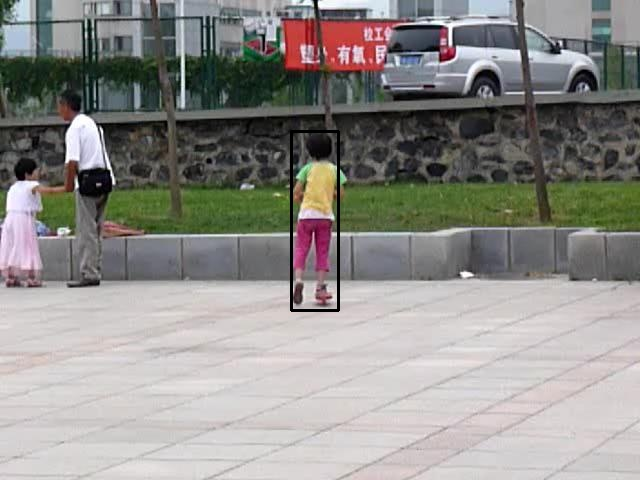
\includegraphics[width = 2.5in]{figures/results/ch_detector/results_girl/frame}} &
        \subfloat{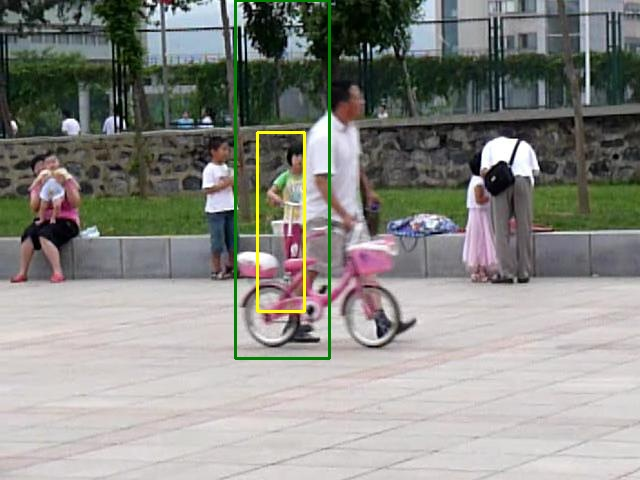
\includegraphics[width = 2.5in]{figures/results/ch_detector/results_girl/result}} \\

        \end{tabular}}
    \caption{Colour co-occurrence histogram detection against occlusion\label{fig:ch_partial_occlusion}
    }
\end{figure}

\section{Mean Shift Tracker}\label{results_mean_shift_tracker}
This Section deals with the qualitative and quantitative analysis of the mean
shift tracker (MST) performance as implemented in
Section~\ref{implementation_mean_shift_tracker}. The analysis is broken down
into a set of experiments each dealing with a different image sequence of
interest.

There are generally three parameters that a user can vary when using the MST
\begin{itemize}
    \item $\epsilon$ - step size bounding maximum mean shift vector magnitude
    \item $m$ - bin count of histograms
    \item $(h_x,h_y)$ - kernel dimensions and positioning around or on object
\end{itemize}
We subsequently assess the performance of the MST implementation
for varying parameters $\epsilon$ and $m$ for the sequence in order to see the
effect their on tracker performance, the goal being to select reasonable values
for the two parameters to asses the general practical performance of the MST. 

We perform this assessment as a series of experiments, each of which is based on an image
sequence that exhibits one or more of the challenges to motion tracking
outlined in Section~\ref{literature_review_challenges}. 
The quantitative analysis is in terms of the tracker error metric over the whole
sequence. The qualitative analysis is based of snapshots of the frames
exhibiting the particular challenge.

\subsection{Effect of step size, $\epsilon$}\label{results_eps}
The parameter $\epsilon$ defines the maximum allowable mean shift step. The
effect of $\epsilon$ on tracker performance varies and is not quantified easily.
A larger $\epsilon$ can make the MST more robust to occlusions to objects in
translation meaning the new center can jump past the occlusion, an example of
this could be a pedestrian walking past a telephone mast. On the other hand,
if the step is too large the tracker response will ``jitter'' due to the
choosing of suboptimal locations for the location of new object position, as it
would skip the necessary iterative refinement step to pick the position that best
matches the model PDF\@. 
The trade-off in the selection of the MST parameter $\epsilon$ is between faster
execution and accuracy.
Furthermore, as addressed later, $\epsilon$ can encode a level of robustness to some challenges such
as target speed and occlusion. 

\subsection{Effect of bin count, $m$}\label{results_m}
This experiment aims to quantitatively determine the effect of varying the
bin count, $m$ on the execution time of calculating the histogram, and computing
the Bhattacharyya coefficient.

The setup is simple enough, the execution time of the \lstinline{get_pdf ()} and
\lstinline{get_BC ()} functions was averaged over 1000 iterations for varying
values of m for a template of dimensions (100,100).

The effect of varying $m$ on histogram generation is shown in
Figure~\ref{fig:results_m_pdf}. There is not significant trend shown between the
bin count and the execution time of the \lstinline{get_pdf ()} function. This makes sense
because we still iterate over all the pixels to allocate each of them to a
particular bin. The access time of the bins in the underlying \textbf{NumPy} array is not
a significant bottle neck for array sizes (bin counts) ranging 1 to 256.

The effect of varying the $m$ on the calculation of the Bhattacharyya coefficient is
detailed in Figure~\ref{fig:results_m_bc}. The execution time of the
\lstinline{get_BC ()} goes  

\Figure[width=0.7\columnwidth]{Graph showing effect of bin size (m) on execution time (ms) of \lstinline{get\_pdf()}}{results/mean_shift_tracker/results_m_pdf}

\Figure[width=0.7\columnwidth]{Graph showing effect of bin size (m) on execution time (ms) of \lstinline{get\_BC()}}{results/mean_shift_tracker/results_m_bc}

The experiments 1-3 aim to assess performance of the MST in dealing with the
various motion tracking challenges, for varying sizes of kernel initialisation.
The general idea is to compare the performance of a large kernel (yellow)
encompassing the whole object of interest, and a smaller kernel (green), that is
initialised around some feature of the larger object. 

For the subsequent experiments, the parameters $\epsilon$ and $m$ of the MST are
kept constant as $\epsilon=5$ and $m=8$. These choices were informed by the
discussions and results in Sections~\ref{results_eps} and~\ref{results_m}. 

\subsection{Experiment 1: fish}
This sequence is one in which there are several fish, of which a distinctly yellow fish is
tracked. The challenges to motion tracking that arise in this image sequence are the following.
\begin{itemize}
    \item occlusion/track overlap
    \item Scaling 
\end{itemize}

The graph in Figure~\ref{fig:results/mean_shift_tracker/fish3/metric} shows the
performance of the MST according to the tracker error metric.
The motion tracking challenges present within the sequence are highlighted
between vertical bars, with the partial occlusion/track overlap challenge and the changing orientation challenge occurring in the green domain.
Reference to the graph is made in the treatment of the discussion of the
particular challenges that follows.

\Figure[width=0.8\columnwidth]{Graph of tracker error of MST (pixels) vs frames in fish sequence}{results/mean_shift_tracker/fish3/metric}

\subsubsection{Partial occlusion}\label{mean_shift_partial_occlusion}
The relevant subsequence exhibiting partial occlusion ranges from
$\mathbf{f}_{178}$ to $\mathbf{f}_{240}$ of the original sequence. 

This interval is represented by the orange domain of the graph in
Figure~\ref{fig:results/mean_shift_tracker/fish3/metric}. From the graph it can be
seen that the mean shift tracker actually performs better under occlusion than in
some other sub sequences that exhibit motion, the average error between the
tracker centroid and the ground truth centroids in this region is around 5
pixels, part of which could also be attributed to different initialisations for
the fish tracker and the regions defining the ground truths.

In Figure~\ref{fig:mean_shift_partial_occlusion} Our target, the yellow fish
remains stationary from $\mathbf{F_{1}}$ to $\mathbf{F_{16}}$. Both kernels are
unaffected by the second gray fish, occupying the same pixel space as our
target. 

Both the metric and the image frames suggest that the MST is relatively robust
to partial occlusion and track overlap in the fish sequence. This is due to the fact that the target
fish and the second fish are easily distinguishable within the RGB colour-space
from which we derive our histograms. Therefore, the tracker is not drawn to the
second fish. As we still partially see a large part of our target when
occluded, our similarity, $\rho$ at the should remain greatest at the position
of the target despite the partial occlusion, which seems to be the case as the
tracker does not drift.

\begin{figure}     
    \makebox[\linewidth][c]{
    \begin{tabular}{cccc}
        \subfloat{\includegraphics[width = 1.5in]{figures/results/mean_shift_tracker/fish3/occlusion/1.jpg}} &
        \subfloat{\includegraphics[width = 1.5in]{figures/results/mean_shift_tracker/fish3/occlusion/2.jpg}} &
        \subfloat{\includegraphics[width = 1.5in]{figures/results/mean_shift_tracker/fish3/occlusion/3.jpg}} &
        \subfloat{\includegraphics[width = 1.5in]{figures/results/mean_shift_tracker/fish3/occlusion/4.jpg}} \\

        \subfloat{\includegraphics[width = 1.5in]{figures/results/mean_shift_tracker/fish3/occlusion/5.jpg}} &
        \subfloat{\includegraphics[width = 1.5in]{figures/results/mean_shift_tracker/fish3/occlusion/6.jpg}} &
        \subfloat{\includegraphics[width = 1.5in]{figures/results/mean_shift_tracker/fish3/occlusion/7.jpg}} &
        \subfloat{\includegraphics[width = 1.5in]{figures/results/mean_shift_tracker/fish3/occlusion/8.jpg}} \\
       
        \subfloat{\includegraphics[width = 1.5in]{figures/results/mean_shift_tracker/fish3/occlusion/9.jpg}} &
        \subfloat{\includegraphics[width = 1.5in]{figures/results/mean_shift_tracker/fish3/occlusion/10.jpg}} &
        \subfloat{\includegraphics[width = 1.5in]{figures/results/mean_shift_tracker/fish3/occlusion/11.jpg}} &
        \subfloat{\includegraphics[width = 1.5in]{figures/results/mean_shift_tracker/fish3/occlusion/12.jpg}} \\
       
        \subfloat{\includegraphics[width = 1.5in]{figures/results/mean_shift_tracker/fish3/occlusion/13.jpg}} &
        \subfloat{\includegraphics[width = 1.5in]{figures/results/mean_shift_tracker/fish3/occlusion/14.jpg}} &
        \subfloat{\includegraphics[width = 1.5in]{figures/results/mean_shift_tracker/fish3/occlusion/15.jpg}} &
        \subfloat{\includegraphics[width = 1.5in]{figures/results/mean_shift_tracker/fish3/occlusion/16.jpg}} \\   

        \end{tabular}}
    \caption{Challenge: partial occlusion\label{fig:mean_shift_partial_occlusion}
 }
\end{figure}

\subsubsection{Changing orientation}
The relevant subsequence exhibiting the challenge of ranges from
$\mathbf{f}_{430}$ to $\mathbf{f}_{512}$ of the fish sequence.  

This interval is represented by the green domain of the graph in
Figure~\ref{fig:results/mean_shift_tracker/fish3/metric}. From the graph it can be
seen that the mean shift tracker actually performs better when faced with this
challenge than it does in the sub sequences that exhibit motion, the average
tracker error between the tracker centroid and the ground truth centroids in
this region is around 5 pixels. 

\begin{figure}     
    \makebox[\linewidth][c]{
    \begin{tabular}{cccc}
        \subfloat{\includegraphics[width = 1.5in]{figures/results/mean_shift_tracker/fish3/orientation/1.jpg}} &
        \subfloat{\includegraphics[width = 1.5in]{figures/results/mean_shift_tracker/fish3/orientation/2.jpg}} &
        \subfloat{\includegraphics[width = 1.5in]{figures/results/mean_shift_tracker/fish3/orientation/3.jpg}} &
        \subfloat{\includegraphics[width = 1.5in]{figures/results/mean_shift_tracker/fish3/orientation/4.jpg}} \\

        \subfloat{\includegraphics[width = 1.5in]{figures/results/mean_shift_tracker/fish3/orientation/5.jpg}} &
        \subfloat{\includegraphics[width = 1.5in]{figures/results/mean_shift_tracker/fish3/orientation/6.jpg}} &
        \subfloat{\includegraphics[width = 1.5in]{figures/results/mean_shift_tracker/fish3/orientation/7.jpg}} &
        \subfloat{\includegraphics[width = 1.5in]{figures/results/mean_shift_tracker/fish3/orientation/8.jpg}} \\
       
        \subfloat{\includegraphics[width = 1.5in]{figures/results/mean_shift_tracker/fish3/orientation/9.jpg}} &
        \subfloat{\includegraphics[width = 1.5in]{figures/results/mean_shift_tracker/fish3/orientation/10.jpg}} &
        \subfloat{\includegraphics[width = 1.5in]{figures/results/mean_shift_tracker/fish3/orientation/11.jpg}} &
        \subfloat{\includegraphics[width = 1.5in]{figures/results/mean_shift_tracker/fish3/orientation/12.jpg}} \\
       
        \subfloat{\includegraphics[width = 1.5in]{figures/results/mean_shift_tracker/fish3/orientation/13.jpg}} &
        \subfloat{\includegraphics[width = 1.5in]{figures/results/mean_shift_tracker/fish3/orientation/14.jpg}} &
        \subfloat{\includegraphics[width = 1.5in]{figures/results/mean_shift_tracker/fish3/orientation/15.jpg}} &
        \subfloat{\includegraphics[width = 1.5in]{figures/results/mean_shift_tracker/fish3/orientation/16.jpg}} \\   

        \end{tabular}}
    \caption{Challenge: changing orientation\label{fig:mean_shift_orientation}
 }
\end{figure}

Experiment 1 shows that the MST is relatively robust to both partial occlusion and changing
object orientation for objects that are easily distinguishable from their
backgrounds backgrounds and occlusions within the chosen low-level feature space.

\subsection{Experiment 2: girl}
This sequence is one of a girl in a park riding around on a scooter. She is
wearing a distinctive colourful outfit relative to the rest of the moving objects in the
scene, which consists mostly of other humans.
The relevant challenges presented in this scene are:
\begin{itemize}
    \item Occlusion (complete)
    \item Scaling 
    \item Ego motion  
\end{itemize}

Ego motion is present through out the scene as the camera follows the girl, the
effect of this on the tracker performance is hard to quantify. The results and
analysis of the challenges of complete occlusion and scaling are subsequently
presented.

The graph in Figure~\ref{fig:results/mean_shift_tracker/girl/metric} shows the
performance of the MST throughout the girl sequence according to the average error metric outlined in
Section~\ref{methodology_testing}.  

\Figure[width=0.8\columnwidth]{Graph of tracker error of MST (pixels) vs frames in girl sequence}{results/mean_shift_tracker/girl/metric}

\subsubsection{Complete occlusion}
The relevant subsequence exhibiting complete occlusion ranges from $\mathbf{f}_{97}$ to
$\mathbf{f}_{127}$ in the original sequence. This range corresponds to 
the orange domain of the graph in
Figure~\ref{fig:results/mean_shift_tracker/girl/metric}. To visualise the
challenge, a set of equally spaced snapshots for the subsequence exhibiting complete occlusion
are presented in Figure~\ref{fig:mean_shift_complete_occlusion}.

\begin{figure}    
    \makebox[\linewidth][c]{
    \begin{tabular}{cccc}
        \subfloat{\includegraphics[width = 1.5in]{figures/results/mean_shift_tracker/girl/occlusion/1.jpg}} &
        \subfloat{\includegraphics[width = 1.5in]{figures/results/mean_shift_tracker/girl/occlusion/2.jpg}} &
        \subfloat{\includegraphics[width = 1.5in]{figures/results/mean_shift_tracker/girl/occlusion/3.jpg}} &
        \subfloat{\includegraphics[width = 1.5in]{figures/results/mean_shift_tracker/girl/occlusion/4.jpg}} \\

        \subfloat{\includegraphics[width = 1.5in]{figures/results/mean_shift_tracker/girl/occlusion/5.jpg}} &
        \subfloat{\includegraphics[width = 1.5in]{figures/results/mean_shift_tracker/girl/occlusion/6.jpg}} &
        \subfloat{\includegraphics[width = 1.5in]{figures/results/mean_shift_tracker/girl/occlusion/7.jpg}} &
        \subfloat{\includegraphics[width = 1.5in]{figures/results/mean_shift_tracker/girl/occlusion/8.jpg}} \\
       
        \subfloat{\includegraphics[width = 1.5in]{figures/results/mean_shift_tracker/girl/occlusion/9.jpg}} &
        \subfloat{\includegraphics[width = 1.5in]{figures/results/mean_shift_tracker/girl/occlusion/10.jpg}} &
        \subfloat{\includegraphics[width = 1.5in]{figures/results/mean_shift_tracker/girl/occlusion/11.jpg}} &
        \subfloat{\includegraphics[width = 1.5in]{figures/results/mean_shift_tracker/girl/occlusion/12.jpg}} \\
       
        \subfloat{\includegraphics[width = 1.5in]{figures/results/mean_shift_tracker/girl/occlusion/13.jpg}} &
        \subfloat{\includegraphics[width = 1.5in]{figures/results/mean_shift_tracker/girl/occlusion/14.jpg}} &
        \subfloat{\includegraphics[width = 1.5in]{figures/results/mean_shift_tracker/girl/occlusion/15.jpg}} &
        \subfloat{\includegraphics[width = 1.5in]{figures/results/mean_shift_tracker/girl/occlusion/16.jpg}} \\   

        \end{tabular}
    }
    \caption{Challenge: complete occlusion\label{fig:mean_shift_complete_occlusion}}
\end{figure}

It is apparent by the large spike in tracker error over the orange domain, that
the MST deals poorly with the challenge of complete occlusion.  This is expected
as the implementation of the MST is based on visual low-level features of the
RGB colour space. It does however relocate the girl relatively fast after the
occlusion ends, but it this would not necessarily be the case in sequences exhibiting 
longer occlusion periods as this could allow the tracker to drift too far to
relocate the target model. 

Figure~\ref{fig:mean_shift_complete_occlusion} provides visual insight into
what is going on. Snapshots $\mathbf{F}_4$ to $\mathbf{F}_{13}$ show that the
MST is able to relocate the girl within after a man completely occludes her. We
see that the smaller green kernel is offset by man for a bit, whereby the larger
yellow kernel remains relatively stable. The green kernel behaviour can be
explained by the fact that it's model, $\hat{q}$ was defined solely around the
Girl's yellow top. This is sufficiently close for the man's white top within the
RGB colour-space to cause a small drift in the kernel which lasts only until the
girl is visible again upon which the tracker is pulled back towards the girl as
she is the once again the local maximum of our similarity measure $\rho$.

\subsubsection{Scaling}
The challenge of scaling is exhibited from $\mathbf{f}_{427}$ to
$\mathbf{f}_{997}$ in the original sequence, where the girl is walking away from
the camera, the result being that her dimensions within the frame are becoming
smaller.

The scaling challenge occurs within the green domain of the graph in
Figure~\ref{fig:results/mean_shift_tracker/girl/metric}, 
While the MST tracker error fluctuates significantly between lows of close to 0
and highs of around 40 pixels. The average challenge error for this subsequence
(indicated in purple) is indistinguishable from the average tracker error for the overall girl
sequence (indicated in red).

A set of representative visual snapshot of the of the tracker results for both initialised kernels
for the scaling subsequence are presented in
Figure~\ref{fig:mean_shift_girl_scale}. It shows that the girl is successfully
tracked until the completion of the sequence by both the initialised kernels.
The robustness is likely in part due to the distinct nature of her attire when
compared to the rest of the scene. It should be noted that the smaller kernel
seems to perform better than the larger kernel, this cannot however be
quantified by the metric because ground values would be misleading if compared
to an initialisation that is not around the whole target object.

\begin{figure} 
    \makebox[\linewidth][c]{
    \begin{tabular}{cccc}
        \subfloat{\includegraphics[width = 1.5in]{figures/results/mean_shift_tracker/girl/scale/1.jpg}} &
        \subfloat{\includegraphics[width = 1.5in]{figures/results/mean_shift_tracker/girl/scale/2.jpg}} &
        \subfloat{\includegraphics[width = 1.5in]{figures/results/mean_shift_tracker/girl/scale/3.jpg}} &
        \subfloat{\includegraphics[width = 1.5in]{figures/results/mean_shift_tracker/girl/scale/4.jpg}} \\

        \subfloat{\includegraphics[width = 1.5in]{figures/results/mean_shift_tracker/girl/scale/5.jpg}} &
        \subfloat{\includegraphics[width = 1.5in]{figures/results/mean_shift_tracker/girl/scale/6.jpg}} &
        \subfloat{\includegraphics[width = 1.5in]{figures/results/mean_shift_tracker/girl/scale/7.jpg}} &
        \subfloat{\includegraphics[width = 1.5in]{figures/results/mean_shift_tracker/girl/scale/8.jpg}} \\
       
        \subfloat{\includegraphics[width = 1.5in]{figures/results/mean_shift_tracker/girl/scale/9.jpg}} &
        \subfloat{\includegraphics[width = 1.5in]{figures/results/mean_shift_tracker/girl/scale/10.jpg}} &
        \subfloat{\includegraphics[width = 1.5in]{figures/results/mean_shift_tracker/girl/scale/11.jpg}} &
        \subfloat{\includegraphics[width = 1.5in]{figures/results/mean_shift_tracker/girl/scale/12.jpg}} \\
       
        \subfloat{\includegraphics[width = 1.5in]{figures/results/mean_shift_tracker/girl/scale/13.jpg}} &
        \subfloat{\includegraphics[width = 1.5in]{figures/results/mean_shift_tracker/girl/scale/14.jpg}} &
        \subfloat{\includegraphics[width = 1.5in]{figures/results/mean_shift_tracker/girl/scale/15.jpg}} &
        \subfloat{\includegraphics[width = 1.5in]{figures/results/mean_shift_tracker/girl/scale/16.jpg}} \\   
    \end{tabular}}
    \caption{Challenge: scale change\label{fig:mean_shift_girl_scale}}
\end{figure}

\subsection{Experiment 3: ants}
This image sequence is of multiple ants in motion within a Petri dish. The Ants
are almost identical, with some being marked by a colourful mark on the abdomen
to likely help distinguish them in analysis.

The challenges presented by this sequence are the following:
\begin{itemize}
    \item Target speed
    \item Track overlap
\end{itemize}

The graph in Figure~\ref{fig:results/mean_shift_tracker/girl/metric} shows the
performance of the MST over the ant sequence according to the average error metric outlined in
Section~\ref{methodology_data_analysis}.  

\Figure[width=0.8\columnwidth]{Graph of tracker error of adaptive tracker (pixels) vs frames in ant sequence}{results/mean_shift_tracker/ants/metric}


\subsubsection{Track Overlap}\label{mean_shift_track_overlap}
This Challenge is exhibited in $\mathbf{f}_{214}$ to $\mathbf{f}_{240}$ in the
original ant image sequence. The sequence h two ants coming within close proximity of
each other, we can see that the yellow kernel switches to track the second Ant
after the crossing of their tracks within the sequence. Let us refer to the
original ant as $A_0$ and the second ant as $A_1$. 

Figure~\ref{fig:mean_shift_ant_speed} presents a set of representative snapshots
for the tracker results for the subsequence exhibiting the challenge of track
overlap.

\begin{figure}
    \makebox[\linewidth][c]{
    \begin{tabular}{cccc}
        \subfloat{\includegraphics[width = 1.5in]{figures/results/mean_shift_tracker/ants/speed/1.jpg}} &
        \subfloat{\includegraphics[width = 1.5in]{figures/results/mean_shift_tracker/ants/speed/2.jpg}} &
        \subfloat{\includegraphics[width = 1.5in]{figures/results/mean_shift_tracker/ants/speed/3.jpg}} &
        \subfloat{\includegraphics[width = 1.5in]{figures/results/mean_shift_tracker/ants/speed/4.jpg}} \\

        \subfloat{\includegraphics[width = 1.5in]{figures/results/mean_shift_tracker/ants/speed/5.jpg}} &
        \subfloat{\includegraphics[width = 1.5in]{figures/results/mean_shift_tracker/ants/speed/6.jpg}} &
        \subfloat{\includegraphics[width = 1.5in]{figures/results/mean_shift_tracker/ants/speed/7.jpg}} &
        \subfloat{\includegraphics[width = 1.5in]{figures/results/mean_shift_tracker/ants/speed/8.jpg}} \\
       
        \subfloat{\includegraphics[width = 1.5in]{figures/results/mean_shift_tracker/ants/speed/9.jpg}} &
        \subfloat{\includegraphics[width = 1.5in]{figures/results/mean_shift_tracker/ants/speed/10.jpg}} &
        \subfloat{\includegraphics[width = 1.5in]{figures/results/mean_shift_tracker/ants/speed/11.jpg}} &
        \subfloat{\includegraphics[width = 1.5in]{figures/results/mean_shift_tracker/ants/speed/12.jpg}} \\
       
        \subfloat{\includegraphics[width = 1.5in]{figures/results/mean_shift_tracker/ants/speed/13.jpg}} &
        \subfloat{\includegraphics[width = 1.5in]{figures/results/mean_shift_tracker/ants/speed/14.jpg}} &
        \subfloat{\includegraphics[width = 1.5in]{figures/results/mean_shift_tracker/ants/speed/15.jpg}} &
        \subfloat{\includegraphics[width = 1.5in]{figures/results/mean_shift_tracker/ants/speed/16.jpg}} \\   
    \end{tabular}}
    \caption{Challenge: target speed: small kernel loses blue ant\label{fig:mean_shift_ant_speed}}
\end{figure}

From the graph in Figure~\ref{fig:results/mean_shift_tracker/girl/metric},
it can be seen that for $\mathbf{f}_0$ to $\mathbf{f}_{214}$ where the blue
target ant is exhibiting relatively slow motion, the tracker error fluctuates
around the 10 pixel region. Upon reaching the challenge of track overlap over
frames $\mathbf{f}_{214}$ to $\mathbf{f}_{240}$, the tracker clearly fails, as
evidenced by the continual rise in tracker error beyond this region.

Upon inspection of the snapshots of the track overlap subsequence presented in
Figure~\ref{fig:mean_shift_ant_speed}, snapshots $\mathbf{F}_5$ to
$\mathbf{F}_{11}$, highlight that the yellow kernel begins to track the yellow
ant in place of the original blue ant target. At this point the tracker has
failed.

It is important at this point to highlight the differences between this case of
track overlap, and that detailed in Section~\ref{mean_shift_partial_occlusion},
in which, despite the tracks for the yellow fish and grey fish overlapping
entirely, the tracker remains remains unaffected.
The answer lies within the feature space our tracker is based on. Within the RGB colour space,
the yellow and grey fish are largely distinct. Hence the tracker will not be
drawn to the grey fish as it exits the yellow kernel.

In this case, the are two objects within the vicinity of yellow kernel that are practically
indistinguishable within our chosen feature space. As the blue ant quickly exits
the Kernel, the gradient within the domain of the similarity
function is not sufficiently steep to draw the tracker away.

With $A_b$ and $A_y$ close to each other, The fact that $A_b$ moves with a high
velocity, $A_b$ between $\mathbf{f}_k$ and $\mathbf{f}_{k+1}$ is easily be large
enough to place $A_y$ closer to $A_b$ in $\mathbf{f}_{k+1}$, which makes the
mean shift vector point to $A_{y}$ as the local maxima in the domain of the
similarity function thus the MST latches onto $A_y$ as the it new location in
$\mathbf{f}_{k+1}$.

\subsubsection{Target speed}\label{mean_shift_target_speed}
The smaller green kernel is continually affected by this challenge throughout
the ant image sequence.
For the larger yellow kernel the relevant subsequence exhibiting the challenge
of target speed occurs within $\mathbf{f}_{256}$ and $\mathbf{f}_{277}$ of in
the original sequence. 
Since the tracker has changed tracks from the blue to the yellow ant before
reaching this challenge, the graph of tracker error against frame presented in
Figure~\ref{fig:results/mean_shift_tracker/girl/metric} is of no use because
the subsequent ground truth values correspond to the blue ant and not the yellow
ant that the MST is centred on. Subsequent analysis aims to highlight the effect
of kernel size when faced with the challenge of high target speed.

Beginning with the smaller green kernel.
Figure~\ref{fig:mean_shift_ant_speed}, presents representative snapshots. 
It is apparent that the green kernel barely moves to track any of the ants it is
centred on throughout the ant sequence. A proposed explanation for this
observation ties back to sampling theory and knowledge of the mean shift
procedure as defined in Section~\ref{theoretical_framework_mean_shift_tracker}.

Keeping in mind that a digital video is a sampling of an analogue scene.
In order to discuss the effect of the ``speed'' of a target on tracker
performance it is necessary to interpret this speed more clearly
as the magnitude of an object's inter-frame displacement, $\mathbf{\delta}$ - which
we define as the distance between an object's
position between two adjacent frames $\mathbf{f}_k$ and $\mathbf{f}_{k+1}$.
This is an adequate formulation because, depending on the sampling frequency $f_s$ of
a particular sequence, a fast object such as a car sampled at a high $f_s$ can
have a smaller $\mathbf{\delta}$ than a relatively slow snail sampled at a lower
$f_s$~\cite{Tekalp2014}. 

As the $\delta$ of an object between $\mathbf{f}_k$ and $\mathbf{f}_{k+1}$ 
increases in magnitude, less of the object lies within the dimensions
$(h_x,h_y)$ of the kernel that we initialise at it's last known pixel location
$\mathbf{c_0}$ in $\mathbf{f}_k$. In terms of the mean shift tracking algorithm this simply
results in a larger mean shift vector, $\vec{m}$. That said, the initialised green kernel
throughout Figure~\ref{fig:mean_shift_ant_speed} highlights the extreme case in
which the kernel initialised at the last known target location $\mathbf{c_0}$
from $\mathbf{f}_{k}$ does not even partly contain the target in
$\mathbf{f}_{k+1}$.

Within the overall ant sequence, the performance of the larger yellow kernel in
tracking the blue ant is consistent until faced with the challenge
of track overlap, 

Figure~\ref{fig:mean_shift_ant_speed2} shows snapshots from $\mathbf{f}_{265}$ to
$\mathbf{f}_{277}$ of the original sequence. It highlights the fact that even the larger
yellow kernel is not completely robust to the challenge of high target speed. 

\begin{figure}
    \makebox[\linewidth][c]{
    \begin{tabular}{cccc}
        \subfloat{\includegraphics[width = 1.5in]{figures/results/mean_shift_tracker/ants/speed2/1.jpg}} &
        \subfloat{\includegraphics[width = 1.5in]{figures/results/mean_shift_tracker/ants/speed2/2.jpg}} &
        \subfloat{\includegraphics[width = 1.5in]{figures/results/mean_shift_tracker/ants/speed2/3.jpg}} &
        \subfloat{\includegraphics[width = 1.5in]{figures/results/mean_shift_tracker/ants/speed2/4.jpg}} \\
    \end{tabular}}
    \caption{Challenge: target speed: large kernel loses ant\label{fig:mean_shift_ant_speed2}}
\end{figure}

The snapshots presented in Figure~\ref{fig:mean_shift_ant_speed} tell us
that a larger kernel larger kernel size is more robust to the effects of large
$\mathbf{\delta}$ than the smaller green kernel. However, as
Figure~\ref{fig:mean_shift_ant_speed2} presents, even a larger
kernel enclosing the whole object of interest can lose track of the object given
a sufficiently large $\mathbf{\delta}$, for which the target object in $\mathbf{f}_{k+1}$ lies
to far from it's last known location $\mathbf{c_0}$ in $\mathbf{f}_k$, as was
the case for the smaller green kernel. 

In looking for a solution to this issue, it is important to note that increasing
our kernel size largely beyond the object dimensions is clearly not a feasible solution
for dealing with this challenge, as it would incorporate a lot of noise into the
object model $\hat{q}$, likely deteriorating tracker performance when faced with
other motion tracking challenges.

As discussed in subsection~\ref{results_eps}, The MST parameter, $\epsilon$ has
the potential to increase the MST's robustness to challenges such as target
speed and occlusion, at the cost of increased track ``jitter''. 

One approach to to the problem can be tied back to the initial sampling rate,
$f_s$ used to obtain the sequence. If a higher sampling rate were used, it would
mean higher redundancy between adjacent frames in the image sequence resulting
in smaller $\mathbf{\delta}$ values. An impractical solution therefore could be to try
and obtain the same sequence again, but sampled at a higher $f_s$.
This is likely unfeasible. Furthermore, one can easily imagine situations in which the
available technology is constrained by factors such as budget, size etc. In such
situations, we would still like to be able to track our object of interest. 

A possible solution could be to augment the basic MST implementation with other
forms ideas from other tracking methodologies originally
presented in Figure~\ref{fig:literaturereview_taxonomy_motion_tracking}. This is
possibility is explored as a possible improvement and avenue for future work in
Subsection~\ref{future_mst}. 


\section{Graphical User Interface}\label{results_gui}
This Section presents the results of the implemented GUI. The presentation is in
terms of functionality relating to the MT system user requirements in
Section~\ref{introduction_user_requirements}.

An overview of implemented GUI system is displayed in
Figure~\ref{fig:gui_integration}. The implementation closely follows the layout of the design in
Figure~\ref{fig:design_gui_mockup} the only differences being a reordering of
the menu bar and additional buttons for more convenient navigation of selected
sequences.

\begin{figure}
    \makebox[\linewidth][c]{
    \begin{tabular}{cc}
        \subfloat{\includegraphics[width = 3in]{figures/results/gui/first_look}} &
        \subfloat{\includegraphics[width = 3in]{figures/results/gui/second_look}} 
    \end{tabular}}
    \caption{Image of integrated MT System on the Ubuntu and OS X operating systems\label{fig:gui_integration}}
\end{figure}

        
\subsection{I/O functionality}
The GUI allows for user selected sequence selection from any file directory on
the system it is being run on.

\subsection{Navigational functionality}.
The GUI implementation provides navigational buttons that provide a user a
standard video sequence interface.

\section{Integration}
This section deals with documenting the integrated MT System

\subsection{Algorithm integration}
The three algorithms discussed in Section~\ref{chapter_theoretical_framework}
successfully integrated with the front-end GUI. A sample use sequence within the GUI is
presented in Figure~\ref{fig:gui_CHD}. This sequence presents the user flow
involved in applying the CCH-detector to a particular frame. This is essentially
the same user flow as the one highlighted by the sequence diagram in
Figure~\ref{implementation_sequence_diagram}. 

\begin{figure}
    \makebox[\linewidth][c]{
    \begin{tabular}{ccc}
        \subfloat{\includegraphics[width = 2.2in]{figures/results/gui/CHD_1.png}} &
        \subfloat{\includegraphics[width = 2.2in]{figures/results/gui/CHD_2.png}} &
        \subfloat{\includegraphics[width = 2.2in]{figures/results/gui/CHD_3.png}} \\
    \end{tabular}}
    \caption{Algorithm user flow\label{fig:gui_CHD}}
\end{figure}

\subsection{Repository}
The integrated MT System is available at the relevant GitHub
repository~\cite{repository}~\footnote{https://github.com/Claude47/thesis\_product}.
The README.md file within the repository provides potential users with a comprehensive guide to
easily installing the MT System and its dependencies within an isolated Python virtual environment.

Upon installation, a user is offered a choice between using the back-end APIs to
integrate the tracker implementations into their own applications or to interact
with the trackers via the GUI interface. 
